\documentclass[12pt,a4paper]{article}
\usepackage[utf8x]{inputenc}
\usepackage{ucs}
\usepackage{amsfonts}
\usepackage{amssymb}
\usepackage{graphicx}
\usepackage{hyperref}
\usepackage[left=2cm,right=2cm,top=2cm,bottom=2cm]{geometry}
\begin{document}

\begin{center}
\begin{LARGE}
UNIVERSIDAD NACIONAL \\
Paradigmas de Programaci\'on \\
Proyecto de Investigaci\'on \\
Prof. Eddy Ramirez \\
David Lobo
Cristian Díaz
\end{LARGE}
\end{center}

\begin{center}
{\Huge{\textbf{\em Problema 3714- Royale with Cheese}}}
\end{center}

\section{Especificación del problema}
El problema trata de realizar una codificaci\'on de una cadena de car\'acteres. En donde se analiza uno por uno los caracteres, creando la codificaci\'on n\'umerica de cada uno de ellos. Si este ya fue revisado, simplemente se sustituye por el n\'umero ya asignado. Al final el programa imprime la codificaci\'on final de la cadena.

\section{Especificaci\'on de entrada: }
La entrada consiste en m\'ultiples casos de prueba. Cada caso de prueba contiene una cadena S con longitud n (1 $\leq$ n $\leq$ 10$\wedge$5) a que identifica una casa en el extraño sistema de numeraci\'on implementado en Amsterdam. La cadena S se forma solo con 26 letras min\'usculas (de a a z).

\section{Especificaci\'on de salida: }
Para cada identificador de una casa en el sistema de numeraci\'on de Amsterdam, tiene que generar una versi\'on codificada de la ID, tal como lo hace habitualmente la polic\'ia. Cada salida va en una l\'inea.

\section{Condiciones del problema: }
El problema contiene una condici\'on para la codificaci\'on final. Esta es, se tiene que sustituir el {\bf 2} por un {\bf 5}, {\bf 6} por un {\bf 9}; as\'i tambi\'en en su rev\'ez el {\bf 5} por un {\bf 2} y un {\bf 9} por el {\bf 6}.

\section{Ejemplo de Entrada y Salida: }
\begin{center}
\begin{tabular}{|*{2}{c|}l r|}
  \hline
  Entrada & Salida \\
  \hline
   abbchocx & 15534239 \\
   maplortycbjce & 1534297861011615 \\
  \hline
\end{tabular}
\end{center}

\section{Resoluci\'on del problema: }
El primer paso es recibir la cadena de car\'acteres. Y se analiza dos vectores auxiliares Vector Letras{\bf (VL)} y Vector Salida {\bf (VS)}.

Al recibir la cadena, se empieza analizar cada uno de los caracteres, se inicializa el VL en donde se va añadiendo si el caracter se encuentra en \'el.  Si el caracter ya existe, simplemente se agrega en el n\'umero de posici\'on en el VS. Hay que tomar en cuenta que durante la codificaci\'on se va realizando el parseo de las posiciones.

Dando como resultado final la cadena codificada.

\subsection{M\'etodo de Parseo:}
\begin{enumerate}
\item Si el n\'umero es mayor o igual a 20, retorna el {\bf n\'umero + 30 }.
\item Si el n\'umero ingresado m\'odulo de 10 es igual 2, retorna el {\bf n\'umero + 3 }.
\item Si el n\'umero ingresado m\'odulo de 10 es igual 6, retorna el {\bf n\'umero + 3 }.
\item Si el n\'umero ingresado m\'odulo de 10 es igual 5, retorna el {\bf n\'umero - 3 }.
\item Si el n\'umero ingresado m\'odulo de 10 es igual 9, retorna el {\bf n\'umero - 3 }.
\item Si no cumple con ninguno de los casos, retorna el {\bf n\'umero }.
\end{enumerate}

\section{Aprobaci\'on de Algoritmo: }
Aprobaci\'on de la p\'agina \textbf{Caribbean Online Judge} \url{http://coj.uci.cu}
\begin{center} 
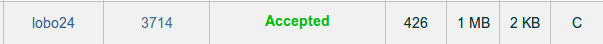
\includegraphics[scale=0.5]{aceptacion}
\end{center}

\section{Soluci\'ones Programadas}
\begin{enumerate}
\item \textbf{\textit{Lenguaje Programaci\'on C}}. \\\\
M\'etodo Principal
\begin{center} 
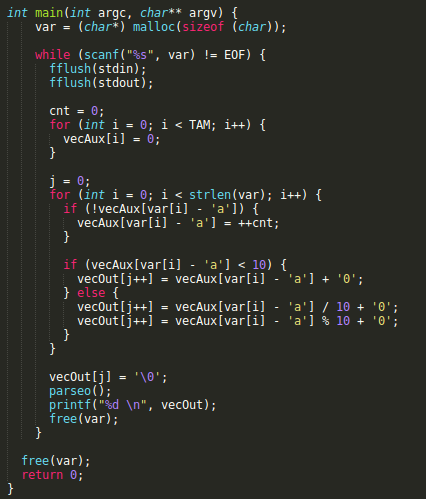
\includegraphics[scale=0.5]{principalC}
\end{center}

M\'etodo Parseo
\begin{center} 
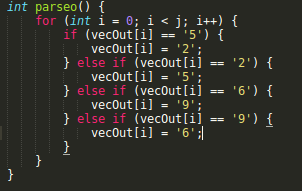
\includegraphics[scale=0.8]{parseoC}
\end{center}

\item \textbf{\textit{Lenguaje Programaci\'on Scheme}}. \\\\
M\'etodo Principal
\begin{center} 
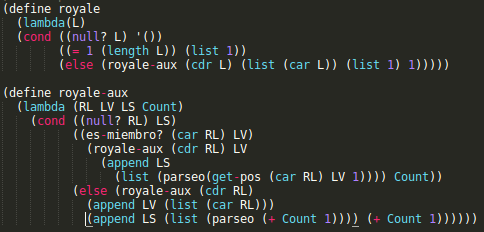
\includegraphics[scale=0.8]{principalScheme}
\end{center}
	
M\'etodo Parseo
\begin{center} 
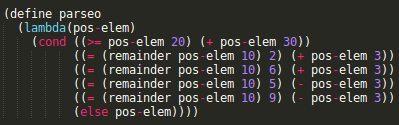
\includegraphics[scale=0.8]{parseoScheme}
\end{center}

M\'etodo devuelve elemento y es miembro
\begin{center} 
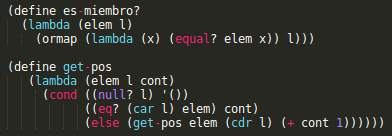
\includegraphics[scale=0.8]{metodosScheme}
\end{center}

\item \textbf{\textit{Lenguaje Programaci\'on Erlang}}. \\\\
M\'etodo Principal
\begin{center}
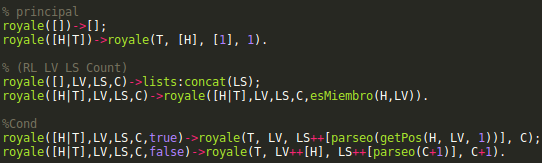
\includegraphics[scale=0.8]{principalErlang}
\end{center}

M\'etodo Parseo
\begin{center}
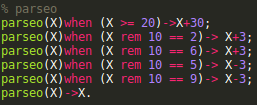
\includegraphics[scale=0.8]{parseoErlang}
\end{center}

M\'etodo devuelve elemento y es miembro
\begin{center}
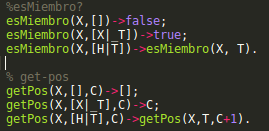
\includegraphics[scale=0.8]{metodosErlang}
\end{center}

\item \textbf{\textit{Lenguaje Programaci\'on Java}}. \\\\
M\'etodo Principal
\begin{center}
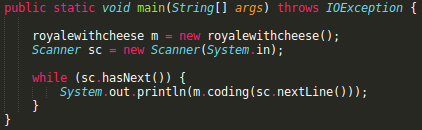
\includegraphics[scale=0.8]{principalJava}
\end{center}

M\'etodo Parseo
\begin{center}
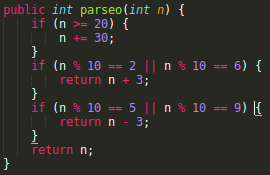
\includegraphics[scale=0.8]{parseoJava}
\end{center}

M\'etodo HashTable
\begin{center}
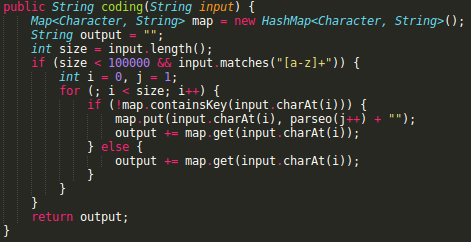
\includegraphics[scale=0.8]{metodoHashJava}
\end{center}

\item \textbf{\textit{Lenguaje Programaci\'on Prolog}}. \\\\
M\'etodo Principal
\begin{center}
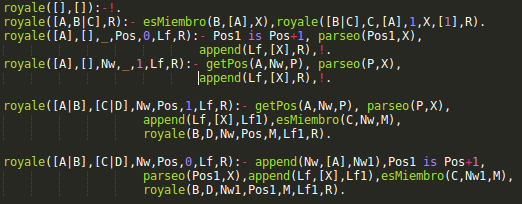
\includegraphics[scale=0.8]{principalProlog}
\end{center}

M\'etodo Parseo
\begin{center}
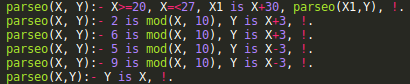
\includegraphics[scale=0.8]{parseoProlog}
\end{center}

M\'etodo devuelve elemento y es miembro
\begin{center}
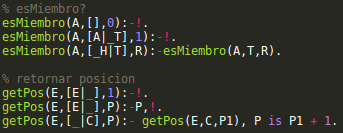
\includegraphics[scale=0.8]{metodosProlog}
\end{center}
\end{enumerate}
\end{document}
